\section{Dihedral intervals and transported reflection orders}
\label{sec:dihedral}

We first establish the plane and graph facts that let an interval
isomorphism transport full relative dihedral intervals. For an edge, a
nonnegative integer attached to each root plane then measures a difference
of later-edge counts; the sum of these integers is half the excess of the
edge's length difference over one. Dyer's reconstruction of dihedral coset
intersections by four-cycle moves \cite[Section~3.4]{Dyer91} precedes the
transport argument needed for the later sheaf comparison.

\subsection{Root planes and relative orders}

We use left reflection labels throughout.  If $\Pi$ is a plane spanned by
two roots, let $D_\Pi$ be the subgroup generated by the reflections whose
roots belong to $\Pi$, and write $\Phi_D^+=\Phi^+\cap\Pi$ for the
induced positive roots.  The following facts distinguish the relative
Bruhat order of a reflection subgroup from the ambient Bruhat order.

\begin{lemma}[Planes and relative orders]\label{dih:plane}
Let $\Pi$ be spanned by two linearly independent roots in the real
realization of $W$.
\begin{enumerate}
\item The subgroup $D=D_\Pi$, with its canonical Coxeter generators,
is dihedral.  Its reflections are exactly the ambient reflections whose
roots lie in $\Pi$.
\item Each coset $D a$ has a unique element $a_0$ of minimal ambient
length.  The map $w\mapsto wa_0$ identifies the labeled directed Bruhat
graph of $D$ with the directed subgraph of the ambient Bruhat graph on
$D a$.  Write $\le_D$ for the resulting relative order and put
\[
 \ell_D(wa_0)=\ell_D(w).
\]
Then $x\le_D y$ implies $x\le y$, and
\[
 \ell_D(x)
 =\#\{\gamma\in\Phi_D^+:x^{-1}\gamma<0\},
 \qquad x\in D a.
\]
\item If a nonidentity element has two factorizations as products of
two distinct reflections, the two pairs of roots span the same plane.
Consequently, all directed two-edge paths with fixed endpoints have
their labels in one maximal dihedral subgroup.
\end{enumerate}
\end{lemma}

\begin{proof}
We use the reflection-subgroup theorem: a reflection subgroup has a
canonical Coxeter system whose simple roots are positive ambient roots
with positive squared lengths and pairwise nonpositive pairings;
see \cite{Deodhar89,Dyer90,Dyer91,Dyer93}.  Every reflection with root in $\Pi$ preserves
$\Pi$ and has the image of its difference from the identity contained
in $\Pi$.  These properties persist under products.  If an ambient
reflection belongs to $D$, its root line, being the image of its
difference from the identity, therefore lies in $\Pi$.

The canonical simple roots of $D$ consequently lie in $\Pi$.  There
cannot be three of them: in the pointed intersection of $\Pi$ with
the ambient positive cone, one of three distinct rays lies strictly
between the other two.  Its root $\gamma$ is a positive linear
combination of the outside roots $\alpha,\beta$.  Pairing this
combination with $\gamma$ would give
\[
 (\gamma,\gamma)
 =c(\gamma,\alpha)+d(\gamma,\beta)\le0,
 \qquad c,d>0,
\]
contrary to its positive squared length.  Since $D$ contains two
distinct reflections with independent root lines, its canonical
rank is exactly two.

Choose an element $a_0$ of least ambient length in $D a$.  For
$\gamma\in\Phi_D^+$, minimality and the reflection length-sign
criterion \eqref{eq:bg-reflection-sign} give $a_0^{-1}\gamma>0$. Thus $a_0^{-1}$ preserves the
signs of all roots of $D$.  For $w\in D$, the signs of
$(wa_0)^{-1}\gamma$ and $w^{-1}\gamma$ agree.  This proves the
inversion-count formula and identifies the orientations and labels
of all relative reflection edges.  Conversely, an ambient reflection
carrying one element of $D a$ to another belongs to $D$, so there are
no further ambient edges on this coset.  The relative graph has a
unique minimum, hence $a_0$ is also the unique ambient-length minimum.
Relative directed paths are ambient directed paths, which proves
the asserted implication between orders. In the finite setting, this is
the coset graph property of \cite[Theorem~1.4]{Dyer91}.

For the final assertion, use the nondegenerate ambient bilinear
space, even when its restriction to $\Pi$ is degenerate.  For
independent roots $\alpha,\beta$, set
\[
 a(v)=\frac{2(v,\alpha)}{(\alpha,\alpha)},
 \qquad
 b(v)=\frac{2(v,\beta)}{(\beta,\beta)}.
\]
The normal forms $a,b$ are independent, and the reflection formula
gives
\[
 (r_\alpha r_\beta-1)v
 =\alpha\bigl(-a(v)+a(\beta)b(v)\bigr)-\beta b(v).
\]
The two coefficient forms are independent as well.  Therefore
\[
 \operatorname{im}(r_\alpha r_\beta-1)
 =\operatorname{span}(\alpha,\beta).
\]
This image depends only on the product.  It gives the common plane
for any other two-reflection factorization, and part~(1) supplies
the maximal dihedral subgroup attached to that plane.  The labels
of a directed two-edge path are distinct, since repeating a
reflection would return to its starting vertex.
\end{proof}

\begin{lemma}[Dihedral interval shape]\label{dih:shape}
Let $D$ be a finite or infinite dihedral Coxeter group, with length
function $\ell_D$ and Bruhat order $\le_D$.  If
$\ell_D(p)<\ell_D(q)$, then $p<_D q$.  For $a<_D c$, put
$n=\ell_D(c)-\ell_D(a)$.  The interval $[a,c]_D$ has one vertex at
each endpoint and two vertices in each internal rank.

For comparable $p<_D q$, there is a directed reflection edge $p\to q$
exactly when $\ell_D(q)-\ell_D(p)$ is odd.  In particular, if $n$ is
even, exactly $n$ directed two-edge paths join $a$ to $c$; if $n$ is
odd, there is no such path.
\end{lemma}

\begin{proof}
Reduced words alternate between the two canonical generators.  In the
infinite group there are two elements of every positive length.  In
$I_2(m)$ there are two elements of each length strictly between $0$ and
$m$, and one element at lengths $0$ and $m$.
The identity is below every element.  At positive shorter length, either
alternating word occurs as a subword of every longer alternating word:
choose the run beginning at its first or second letter.  The subword
criterion \cite[Theorem~2.2.2]{BB05} gives comparability in length order.
At equal length, comparability forces equality.  These facts give the
stated interval shape, including a possible finite longest element as the
singleton top.

An odd alternating reduced word is a palindrome and hence is conjugate
to its middle generator, while every reflection has odd sign.  Thus the
reflections of $D$ are exactly its elements of odd Coxeter length.  For $p<_D q$,
the sign of $qp^{-1}$ is $(-1)^{\ell_D(q)-\ell_D(p)}$, which proves the
left-reflection edge criterion.  A two-edge path must therefore have an
even total rank difference.  If $n=2h>0$, its intermediate vertex may
occupy precisely the $h$ odd offsets $1,3,\ldots,2h-1$.  Each of those
internal ranks has two vertices, giving $2h=n$ paths.
\end{proof}

\begin{remark}\label{dih:relative-paths}
The coset graph identification in Lemma~\ref{dih:plane} transfers these
statements to the relative order in every coset of a maximal plane
subgroup.  This relative order need not be the order induced by all
ambient comparabilities.  What we use is the exact identification of
directed reflection edges.
In particular, if $x<_D c$ has relative length difference two,
Lemma~\ref{dih:shape} gives two relative two-edge paths.  Every ambient
two-edge path from $x$ to $c$ is one of them: its labels lie in the same
maximal plane by Lemma~\ref{dih:plane}(3), and its intermediate vertex
therefore lies in $D x$.
\end{remark}

\subsection{Graph reconstruction from interval order}

The cover relations and rank differences of a Bruhat interval are intrinsic
to its poset. Dyer reconstructed all reflection edges from the covers for
finite Coxeter systems \cite[Proposition~3.3]{Dyer91}. We give a closure
proof for arbitrary Coxeter systems using the plane and shape facts above.

\begin{theorem}[Graph reconstruction]\label{bg:graph}
An isomorphism of Bruhat intervals in arbitrary Coxeter systems preserves
their directed Bruhat graphs. More explicitly, if
$\iota:[u,b]\longrightarrow[u',b']$ is a poset isomorphism, then
\[
 y=tx>x\text{ for a reflection }t
 \quad\Longleftrightarrow\quad
 \iota(y)=t'\iota(x)>\iota(x)\text{ for a reflection }t'.
\]
\end{theorem}

\begin{proof}
For a finite Bruhat interval $Q$, let $\mathcal E_Q$ be the least relation
containing its cover pairs and closed under the following rule. Arrange six
distinct vertices in four layers
\[
 \{a\}\mid\{p,q\}\mid\{r,s\}\mid\{c\}.
\]
If all eight ordered pairs from one layer to the next are in $\mathcal E_Q$,
add $(a,c)$. This rule depends only on the poset.

First suppose that the eight pairs in an application of the rule are actual
directed reflection edges. The two paths from $a$ to $r$ through $p,q$ have
a common root plane by Lemma~\ref{dih:plane}(3). The two labels leaving $a$
are distinct and span that plane. Applying the same argument to the paths
from $a$ to $s$ puts all four middle edges in this plane. The labels of
$p\to r$ and $p\to s$ are again distinct, so the two paths from $p$ to $c$
put the last two labels there as well. Thus all six vertices lie in one
maximal plane coset. By Lemmas~\ref{dih:plane} and~\ref{dih:shape}, the
three edges from $a$ through $p,r$ to $c$ have positive odd relative gaps;
their sum is positive and odd. Lemma~\ref{dih:shape} gives a relative
reflection edge $a\to c$, which
is an ambient edge by Lemma~\ref{dih:plane}. Hence the rule adds only actual
reflection edges.

To prove the converse, we first refine every non-cover reflection edge
$a\xrightarrow{t}c=ta$ to a directed three-edge path in one maximal plane
coset. Its gap is odd, so write $d=d(a,c)\ge3$. We use a consequence of
simple-reflection lifting: for a directed edge $z\xrightarrow{\tau}\tau z$
and a simple reflection $v$, left multiplication gives a directed edge
$vz\to v\tau z$ with label $v\tau v$, unless $\tau=v$.
For a gap at least three, the new gap is at least the old gap minus two and
is positive. For a cover, a reversal would require $vz>z$ and
$v(\tau z)<\tau z$.
The lifting property \cite[Proposition~2.2.7]{BB05} then gives
$z\le v(\tau z)$; their lengths are equal, so $z=v(\tau z)$ and $\tau=v$.
When $\tau=v$, left multiplication indeed swaps the endpoints.

We prove the refinement by induction on $\ell(c)$ in the ambient group.
Choose a simple left descent $v$ of $c$. If $va>a$, then
\[
 a\longrightarrow va\longrightarrow vc\longrightarrow c
\]
is directed: the middle gap is $d-2\ge1$. Its labels are $v,vtv,v$ and lie
in the plane subgroup spanned by the roots of $v$ and $t$. These roots are
independent, since $v=t$ would make the original gap one.

Suppose instead that $va<a$. The edge $va\to vc$ has the same gap $d$ and
an upper vertex of length $\ell(c)-1$. By induction it has a directed path
\[
 w_0=va\longrightarrow w_1\longrightarrow w_2\longrightarrow w_3=vc
\]
whose labels $r_1,r_2,r_3$ lie in a maximal plane subgroup $D$. Its last
label cannot be $v$: that would give $w_2=vw_3=c>w_3$. Nor can both
$r_1,r_2$ equal $v$, since two consecutive uses of $v$ return to the same
vertex. If neither equals $v$, left multiplication by $v$ preserves the
whole directed path, and its labels lie in the conjugate plane subgroup
$vDv$. If $r_1=v$ or $r_2=v$, use instead
\[
 a=vw_0\longrightarrow w_2\longrightarrow w_3\longrightarrow vw_3=c.
\]
Its first edge is respectively the original second edge, because
$vw_0=w_1$, or the $v$-translate of the original first edge, because
$vw_1=w_2$. In the latter case $r_1\ne v$, so that translate is directed.
The last two edges are the original last edge and the upward $v$-edge.
All labels lie in $D$, since $v\in D$ in these cases. This proves the
refinement. Its final path is directed with endpoints $a,c$, so it lies
inside $[a,c]$, even though the descent induction need not stay there.

Now induct on the ambient gap of a reflection edge $a\to c$ inside $Q$.
For gap one it is a cover and belongs to $\mathcal E_Q$. Otherwise choose
the three-edge path just constructed in a maximal plane coset. In
$[a,c]_D$, take both vertices at each of the two internal relative ranks
occupied by this path. Lemma~\ref{dih:shape} supplies these vertices and
all eight reflection edges between the four selected layers, since the
three relative gaps are odd. These edges are ambient edges in
$[a,c]\subseteq Q$ by Lemma~\ref{dih:plane}. Each meets an internal layer,
so its ambient gap is smaller than $d(a,c)$. By induction all eight are in
$\mathcal E_Q$, and the closure rule adds $(a,c)$.

Thus $\mathcal E_Q$ is exactly the directed Bruhat graph of $Q$. A poset
isomorphism preserves covers and the closure rule, hence preserves all
its directed reflection edges. The rule recovers their presence and
direction, without identifying their root labels.
\end{proof}

\subsection{Transport of relative intervals}

We now fix a poset isomorphism
\[
 \iota:[u,b]\longrightarrow[u',b'].
\]
By Theorem~\ref{bg:graph}, it preserves the directed Bruhat graphs of these
intervals.  The next statement recovers all the relative interval
structure that we will need, without requiring labels to be
preserved.

\begin{proposition}[Transport of dihedral intervals]
\label{dih:transport}
Let $D=D_\Pi$ be a maximal root-plane subgroup of $W$.
Suppose $x,c$ belong to a common coset of $D$ and to $[u,b]$, with
$x\le_D c$ and $\ell_D(c)-\ell_D(x)\ge2$.  Then there is a maximal dihedral plane
subgroup $D'$ of $W'$ such that
\[
 \iota\bigl([x,c]_D\bigr)
 =[\iota(x),\iota(c)]_{D'}.
\]
The restricted map preserves and reflects relative order, relative
rank differences, and all directed relative reflection edges.
\end{proposition}

\begin{proof}
Write $n=\ell_D(c)-\ell_D(x)$.  By Lemma~\ref{dih:shape}, the interval
has one vertex at each end, two vertices in every internal rank,
and all possible directed edges between consecutive ranks.  Its
vertices lie in $[u,b]$, by Lemma~\ref{dih:plane}.

The two arrows from $x$ to its relative atoms have distinct labels
after applying $\iota$.  Let $\Pi'$ be the plane of those two root
labels.  For each vertex in the next relative rank, the two paths
through the atoms have the same plane by Lemma~\ref{dih:plane}(3).
Their remaining arrows therefore have labels in $\Pi'$.  Repeat
this argument through the ranks.  More explicitly, if the arrows
into a two-vertex rank have labels in $\Pi'$, choose a vertex of
the preceding rank and form the two paths through these vertices
to each vertex of the following rank.  Their common plane is
$\Pi'$, so the next arrows also lie in that plane.  This proves
that all image vertices lie in one coset of $D'=D_{\Pi'}$.

Consider an original pair of vertices with relative rank
difference two.  By Remark~\ref{dih:relative-paths}, exactly two ambient
directed two-edge paths join them.  Every intermediate vertex of
such a path belongs to $[u,b]$, so graph preservation implies
that their images also have exactly two ambient two-edge paths.

In the target dihedral coset, the two-edge paths imply a positive even
relative rank difference $r$.  Lemma~\ref{dih:shape} gives exactly $r$
relative two-edge paths.  All are ambient paths and lie in $[u',b']$;
conversely, the common-plane property puts every ambient two-edge path
for these endpoints in this coset.  Thus $r=2$.  The two edges of any
such path each have
positive relative rank difference, so both have difference one.

Every consecutive-rank edge of $[x,c]_D$ lies in a consecutive
two-edge path, because $n\ge2$.  Hence every relative cover maps
to a relative cover.  The image endpoints have relative rank
difference $n$, and the image contains two vertices in each
internal relative rank.  These exhaust the full target dihedral
interval.  The comparability and odd-gap criteria in Lemma~\ref{dih:shape}
now show that the restricted map preserves and reflects the relative order
and all reflection edges.
\end{proof}

Figure~\ref{fig:dihedral-transport} illustrates the relative ranks and
reflection edges preserved by the proposition.
\begin{figure}[tbp]
  \centering
  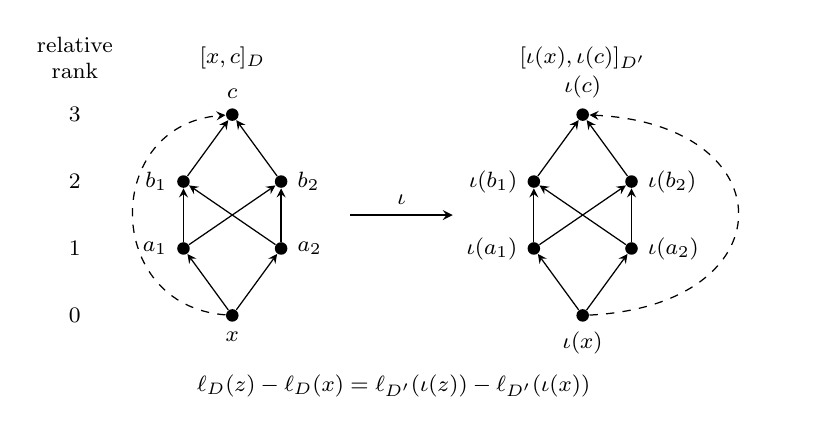
\begin{tikzpicture}[
    x=1cm,y=.85cm,
    font=\footnotesize,
    vertex/.style={circle,fill=black,inner sep=1.6pt},
    cover/.style={->,>=stealth,line width=.45pt},
    longedge/.style={cover,dashed},
    every label/.style={font=\footnotesize}
  ]
    \node[align=center] at (-2.0,3.85) {relative\\rank};
    \foreach \r in {0,1,2,3}
      \node at (-2.0,\r) {$\r$};

    \node at (0,3.85) {$[x,c]_D$};
    \node[vertex,label=below:$x$] (x) at (0,0) {};
    \node[vertex,label=left:$a_1$] (a1) at (-.62,1) {};
    \node[vertex,label=right:$a_2$] (a2) at (.62,1) {};
    \node[vertex,label=left:$b_1$] (b1) at (-.62,2) {};
    \node[vertex,label=right:$b_2$] (b2) at (.62,2) {};
    \node[vertex,label=above:$c$] (c) at (0,3) {};
    \draw[cover] (x)--(a1);
    \draw[cover] (x)--(a2);
    \draw[cover] (a1)--(b1);
    \draw[cover] (a1)--(b2);
    \draw[cover] (a2)--(b1);
    \draw[cover] (a2)--(b2);
    \draw[cover] (b1)--(c);
    \draw[cover] (b2)--(c);
    \draw[longedge] (x) .. controls (-1.65,.15) and (-1.65,2.85) .. (c);

    \begin{scope}[xshift=4.45cm]
      \node at (0,3.85) {$[\iota(x),\iota(c)]_{D'}$};
      \node[vertex,label=below:$\iota(x)$] (ix) at (0,0) {};
      \node[vertex,label=left:$\iota(a_1)$] (ia1) at (-.62,1) {};
      \node[vertex,label=right:$\iota(a_2)$] (ia2) at (.62,1) {};
      \node[vertex,label=left:$\iota(b_1)$] (ib1) at (-.62,2) {};
      \node[vertex,label=right:$\iota(b_2)$] (ib2) at (.62,2) {};
      \node[vertex,label=above:$\iota(c)$] (ic) at (0,3) {};
      \draw[cover] (ix)--(ia1);
      \draw[cover] (ix)--(ia2);
      \draw[cover] (ia1)--(ib1);
      \draw[cover] (ia1)--(ib2);
      \draw[cover] (ia2)--(ib1);
      \draw[cover] (ia2)--(ib2);
      \draw[cover] (ib1)--(ic);
      \draw[cover] (ib2)--(ic);
      \draw[longedge] (ix) .. controls (2.6,.15) and (2.6,2.85) .. (ic);
    \end{scope}

    \draw[->,>=stealth,line width=.6pt]
      (1.5,1.5)--node[above] {$\iota$} (2.8,1.5);
    \node[align=center] at (2.05,-1.05)
      {$\ell_D(z)-\ell_D(x)
        =\ell_{D'}(\iota(z))-\ell_{D'}(\iota(x))$};
  \end{tikzpicture}
  \caption{Transport of a relative dihedral interval of rank three.
    Each internal relative rank contains two vertices.
    The eight solid relative covers give the rank-three instance of the
    closure rule in Theorem~\ref{bg:graph}; the dashed arrow is the recovered
    reflection edge.
    The heights record relative rank differences, not ambient length
    differences, and a relative cover need not be an ambient cover.
    The restriction of $\iota$ preserves these ranks and directed edges;
    no matching of root labels is asserted.}
  \label{fig:dihedral-transport}
\end{figure}


The proposition lets us count within an ordinary dihedral interval in the
second system. The counts therefore depend on its genuine reflection
order, even though the transported order need not be a reflection order
in the first system. We now compute their difference.

\subsection{Later edges and the degree formula}

We first describe the reflection labels in a dihedral group. Let $s,t$ be
its canonical generators. Index the identity by $0$, the alternating word
of length $r$ beginning with $s$ by $r$, and the one beginning with $t$ by
$-r$. For $I_2(m)$ use the representatives $-m<i\le m$ modulo $2m$;
the index $m$ is the longest element. For the infinite group use all
integers. An integer model of the dihedral graph also appears in
\cite[Section~1.10]{DyerRankTwo}. The length of $i$ is $|i|$.

Left multiplication by $s$ and $t$ sends $i$ to $1-i$ and $-1-i$,
respectively. The alternating palindromes with $2n+1$ letters beginning
with $s$ and $t$ therefore act by $i\mapsto a-i$ with parameters
$a=2n+1$ and $a=-(2n+1)$, respectively. These are all the reflections by
Lemma~\ref{dih:shape}, with parameters reduced modulo $2m$ in finite type.
Thus an arrow $i\to j$ has reflection parameter $a=i+j$, its doubled
midpoint.

\begin{lemma}[Midpoint labels and their order]\label{dih:midpoint-order}
Let $D=D_\Pi$ be a maximal plane subgroup in either real realization, with
canonical generators $s,t$ and positive roots $\alpha,\beta$. Choose $h$
positive on the ambient positive roots, as in Section~\ref{sec:background},
and put $\kappa=-(\alpha,\beta)/2\ge0$.
If $D=I_2(m)$, then $\kappa=\cos(\pi/m)$, and the angular order from
$\alpha$ to $\beta$ lists the reflection parameters as
\[
 1\prec3\prec\cdots\prec2m-1\pmod{2m}.
\]
If $D$ is infinite, then $\kappa\ge1$, and that order is
\[
 1\prec3\prec5\prec\cdots
 \prec\cdots\prec-5\prec-3\prec-1.
\]
The geometric construction using $h$ gives this order or its reverse.
\end{lemma}

\begin{proof}
All ambient real roots have squared length $2$, since the action preserves
the form and the simple roots have that length. Define
\[
 p_0=0,\qquad p_1=1,\qquad
 p_{n+1}=2\kappa p_n-p_{n-1}\quad(n\ge1).
\]
For an alternating word of length $n+1$, let $w_n$ be its prefix of length
$n$ and $\sigma_n$ its next letter, with $\alpha_s=\alpha$ and
$\alpha_t=\beta$. The reflection formulas give, by
induction, the two roots $w_n\alpha_{\sigma_n}$
\[
 \delta_n=p_{n+1}\alpha+p_n\beta,\qquad
 \epsilon_n=p_n\alpha+p_{n+1}\beta
\]
for the words beginning with $s$ and $t$, respectively. Their left labels
$w_n\sigma_nw_n^{-1}$ are the alternating palindromes with parameters
$2n+1$ and $-(2n+1)$.

For $0\le n<m$ in finite type and every $n\ge0$ in infinite type, the word
of length $n+1$ is reduced. Its last relative cover is an ambient upward
edge by Lemma~\ref{dih:plane}. The sign criterion
\eqref{eq:bg-reflection-sign} then identifies $\delta_n,\epsilon_n$ as the
positive ambient roots of their
labels. Applying $h$ to both and adding gives
\[
 p_{n+1}+p_n>0
\]
throughout those ranges.

In finite type, the parameter $2m-1$ equals $-1$ modulo $2m$, so
$\delta_{m-1}$ lies on the $\beta$ line and $p_m=0$. If $\kappa\ge1$, the
recurrence instead gives $p_{n+1}>p_n\ge0$ by induction. Thus finite type
has $\kappa<1$. Write $\kappa=\cos\theta$ with $0<\theta\le\pi/2$.
Then
\[
 p_n=\frac{\sin(n\theta)}{\sin\theta},
 \qquad
 p_{n+1}+p_n>0
 \quad\Longleftrightarrow\quad
 \sin\bigl((n+\tfrac12)\theta\bigr)>0.
\]
The equation $p_m=0$ gives $m\theta=j\pi$ for a positive integer $j$.
If $j\ge2$, the first $n$ with $(n+\tfrac12)\theta\ge\pi$ is less than
$m$, and its angle lies in $[\pi,\pi+\theta)\subseteq[\pi,3\pi/2]$.
Its sine is nonpositive, a contradiction. Hence $j=1$ and
$\kappa=\cos(\pi/m)$. In infinite type, $\kappa<1$ would give the same
first sign crossing for some $n$, contradicting positivity for every $n$.
Thus $\kappa\ge1$ there.

The recurrence also gives $p_{n+1}^2-p_np_{n+2}=1$ by induction. Therefore
the slopes $r_n=p_n/p_{n+1}$ of the $\delta_n$ satisfy
\[
 r_{n+1}-r_n=\frac{1}{p_{n+1}p_{n+2}}>0
\]
whenever the denominators are positive. In finite type, the sine formula
makes these slopes increase from $0$ to $+\infty$, ending at $\beta$;
their parameters are all the odd residues $1,3,\ldots,2m-1$. In infinite
type, $p_{n+1}>p_n\ge0$, so the slopes of the $\delta_n$ increase below
$1$, while the reciprocal slopes of the $\epsilon_n$ decrease from
$+\infty$ above $1$. The two families exhaust the reflections. Hence no
other root intervenes, whether their limiting rays coincide or are distinct,
and their slope order is the displayed positive string followed by the
reversed negative string.

Since $h(\alpha),h(\beta)>0$, the normalized point
$(\alpha+r\beta)/h(\alpha+r\beta)$ moves monotonically along the affine
line $h=1$ as the slope $r$ increases. The functional $f$ in the geometric
construction separates the endpoint rays, so $f/h$ gives this order or its
reverse.
\end{proof}

Choose a reflection order in $W'$ and use its labels to schedule
the edges of $[u,b]$: an edge is earlier when its image label is
smaller. Edges with equal image labels are disjoint, so the upward
edges at each fixed vertex are totally ordered without ties.
If they are $e_1,\ldots,e_r$ in increasing schedule order, their
\emph{terminal portions} are the sets $\{e_i,\ldots,e_r\}$
for $1\le i\le r$, together with the empty set. If
$e:x\to y$ is an edge and its root belongs to a plane subgroup
$D$, put
\[
 k_D(e)=\frac{\ell_D(y)-\ell_D(x)-1}{2}.
\]
This is a nonnegative integer by Lemmas~\ref{dih:plane} and~\ref{dih:shape}. The
following identity is the reason that a schedule transported
from another interval suffices.

\begin{lemma}[Later edges in a plane]\label{dih:count}
Let $D$ be a maximal dihedral plane subgroup containing the reflection
that labels an edge $e:x\to y$ of $[u,b]$.
Suppose $y\le_D c$ and $c\in[u,b]$. Let $h_x,h_y$ be the numbers
of outgoing arrows from $x,y$, respectively, in $[x,c]_D$ whose
scheduled labels are strictly later than that of $e$.  Then
\begin{equation}\label{eq:count}
 h_x-h_y=k_D(e).
\end{equation}
\end{lemma}

\begin{proof}
If $[x,c]_D$ has relative rank one, then $c=y$, and both sides
vanish. Otherwise apply $\iota$ using Proposition~\ref{dih:transport}, then
identify the target coset with its dihedral group by Lemma~\ref{dih:plane}.
The transported schedule is now the target label order, and the relative
gaps are unchanged. By the definition of reflection order, this label order
is one of the two angular orders in Lemma~\ref{dih:midpoint-order}.
Rename the resulting group and vertices $D,x,y,c$, and use the integer
indexing above. Lemma~\ref{dih:shape} says that $i\to j$ is an arrow exactly
when
\[
 |i|<|j|\quad\text{and}\quad i-j\ \text{is odd}.
\]
We first use the order starting with $s$; the reversed order will follow
from the count below.

Write $i,j$ for the indices of $x,y$, and put
\[
 L=|i|,\qquad M=|j|,\qquad C=\ell_D(c),
 \qquad k=\frac{M-L-1}{2}.
\]
We use the following midpoint comparison, which we verify after deriving
the count.  Every row concerns only an arrow that exists, so its endpoint
has the required parity and greater absolute length.  In the finite group
$-m$ is omitted because $m$ already represents the longest element.
\begin{center}
\begin{tabular}{c|c|c|c}
starting index&endpoint&
\multicolumn{2}{c}{label is later than that of $i\to j$}
\\
&&$j=M>0$&$j=-M<0$\\ \hline
$i$&$+r$, $r>L$&$r>M$&never\\
$i$&$-r$, $r>L$&always&$r<M$\\
$j$&$+r$, $r>M$&always&never\\
$j$&$-r$, $r>M$&always&never
\end{tabular}
\end{center}
Suppose first that $j=-M$.  The table leaves precisely the negative
endpoints in the eligible ranks strictly between $L$ and $M$.
By Lemma~\ref{dih:shape}, those vertices belong to $[x,c]_D$.
Their ranks form the possibly empty list
\[
 L+1,L+3,\ldots,M-2,
\]
which has $k$ entries.  The table gives no later outgoing arrow at $j$,
so $h_x-h_y=k$.

Now suppose that $j=M$.  The same $k$ negative endpoints below rank $M$
contribute at $i$.  If $c=y$, there are no further contributions.
If $C>M$, the opposite endpoint $-j$ is an internal vertex and contributes
one more later arrow at $i$.  In the finite case $C>M$ implies $M<m$, so
this endpoint is represented.  Put $H=C-M$.  Above rank $M$, all outgoing
arrows from either $i$ or $j$ are later.  At an internal rank $M+t$, the
parity condition permits arrows from $i$ when $t$ is even and from $j$
when $t$ is odd.
The two vertices there therefore contribute $2(-1)^t$ to $h_x-h_y$, while
the singleton top contributes $(-1)^H$.  The total contribution above
rank $M$ is
\[
 2\sum_{t=1}^{H-1}(-1)^t+(-1)^H=-1.
\]
It cancels the extra arrow to $-j$, leaving $h_x-h_y=k$.

For the reversed angular order, Lemma~\ref{dih:shape} shows that the
number of outgoing edges at $a$ in $[a,c]_D$ equals
$\ell_D(c)-\ell_D(a)$: each eligible internal rank contributes two
vertices, and the singleton top contributes when this difference is odd.
The outgoing edges at $y$ in $[x,c]_D$ are exactly those in $[y,c]_D$,
so the total outgoing-edge counts at $x$ and $y$ differ by $2k+1$.
The edge $e$ contributes one at $x$ and none at $y$, and no other edge
incident to $x$ or $y$ has its label.  Removing it and the later arrows leaves an
earlier-arrow difference of $(2k+1)-1-k=k$.  Those arrows are later in
the reversed order.

It remains to verify the midpoint table.  In the infinite group,
$r>|i|$ implies $i+r>0$ and $i-r<0$, while the sign of $i+j$ is the sign
of $j$.  The positive midpoint block precedes the negative block, and
each block is ordered by the ordinary integer order.  Comparing $i+r$
and $i-r$ with $i+j$ gives the two rows starting at $i$.  For arrows from
$j$, use $r>M>|i|$.  If $j=M$, the positive midpoint $M+r$ exceeds $i+M$
and the negative midpoint lies in the later block.  If $j=-M$, the positive
midpoint lies in the earlier block and the negative midpoint $-M-r$ is
smaller than $i-M$.  This gives the other two rows.

In the finite group, a negative midpoint $a$ is represented by $2m+a$.
Comparisons inside one block are unchanged.  For a cross-block arrow from
$i$ when $j=M$, the negative endpoint $-r$ is later because
\[
 2m+i-r>i+M
\]
is equivalent to $r+M<2m$.  This is strict since $r\le m-1$ for a
represented negative endpoint and $M\le m$.  When $j=-M$, a positive
endpoint could be later only if $r+M>2m$, which is impossible since
$r\le m$ and $M\le m-1$.

For arrows starting at $j=M$, the two possible midpoint residues
$M+r$ and $2m+M-r$ exceed $i+M$: the first inequality follows from
$r>|i|$, and the second from $2m-r>i$, using $r\le m$ and $i<m$.
For arrows starting at $j=-M$, the residues $r-M$ and $2m-M-r$ are
smaller than $2m+i-M$: these are respectively $r<2m+i$, using $r\le m$
and $i>-m$, and $-r<i$, using $r>|i|$.  These inequalities include the
possible longest endpoint, so the table has no wrap-around exception.
This completes its verification and the proof.
\end{proof}

The following identity appears in \cite[equation~(1.11.2)]{DyerRankTwo},
with the Bruhat orientation reversed.  We give an inversion-set proof in
the present conventions.

\begin{lemma}[Sum of the planar contributions]\label{dih:sum}
For every arrow $e:x\to y$, the sum over distinct root planes
containing its label satisfies
\begin{equation}\label{eq:sum}
 \sum_D k_D(e)=\frac{d(x,y)-1}{2}.
\end{equation}
Only finitely many summands are nonzero.
\end{lemma}

\begin{proof}
Let $\alpha$ be the positive root of $e$, so that
$y=r_\alpha x$.  For every positive root $\gamma$, set
\[
 \varepsilon(\gamma)
 =\mathbf{1}_{\{y^{-1}\gamma<0\}}
  -\mathbf{1}_{\{x^{-1}\gamma<0\}}.
\]
The two ambient inversion sets are finite, so
$\varepsilon$ has finite support and
\[
 \sum_{\gamma\in\Phi^+}\varepsilon(\gamma)
 =\ell(y)-\ell(x)=d(x,y).
\]
The direction of the arrow gives $x^{-1}\alpha>0$ and
$y^{-1}\alpha<0$, hence $\varepsilon(\alpha)=1$.

Partition the positive roots other than $\alpha$ according
to their planes $\Pi=\operatorname{span}(\alpha,\gamma)$.
By the relative inversion formula in Lemma~\ref{dih:plane},
the contribution of all positive roots in such a plane is
\[
 \sum_{\gamma\in\Phi_D^+}\varepsilon(\gamma)
 =\ell_D(y)-\ell_D(x)=2k_D(e)+1.
\]
Removing $\alpha$ leaves the contribution $2k_D(e)$.
These contributions are nonnegative, and only finitely many
can be nonzero, because each nonzero one meets the finite
support of $\varepsilon$ away from $\alpha$.  Summing the
disjoint parts now gives
\[
 d(x,y)-1=\sum_D 2k_D(e),
\]
as required.  If there is no root independent of $\alpha$,
the sum is empty and the same identity follows directly
from the ambient inversion count.
\end{proof}
